\section{INTRODUCTION}
% バーチャル物体を器用に扱う触覚デバイスは開発途上である
Today anyone can easily construct a virtual reality (VR) environment because of improvements in computer performance and advance in 3D technology such as head mount displays. 
Many VR technologies related to visual and auditory sensations are present in our surroundings and familiar in our lives.
However, the haptic device with which users can intuitively touch the virtual object, recognize the shape of it and dexterously operate it is still under research.

In order to reproduce the haptic information during the interaction between the finger and the virtual object, the haptic device should present the force distribution on the contact surface.
Depending on the shape of the object or frictional characteristics, not only the normal force but also the shear force should be presented to users.
As one of the approaches to reproduce the force distribution, the pin-array display has been developed ~\cite{Shimizu1993}~\cite{Koo2008}.
Though these pin-array devices could present force distribution, the direction of the force was fixed.
For example, most of them were able to present only normal force distributions~\cite{Moy2000,Velazquez2005,Sarakoglou2005,Kim2009}.

% 本研究では...

This study proposes a novel method of presenting force distribution in various directions with the finger mounted pin-array display, in which pins are tilted.
%We present users with the resultant force by summing up the individual forces from pins which tilted differently.
By pairing two pins tilted in different direction, it should be possible to present the resultant force of the two individual forces.
We hypothesize that we can control the felt direction of resultant force by only changing the air pressure applied to each pin (Fig.\ref{fig_intro}).
The method has two advantages.
First, the pin arrangement can be simple as previous pin-array devices and thus, the high density of pins is realized.
Second, it takes little time to change the pressure compared to changing the direction of the actuator itself and thus, the method can change of direction of the presented force with low latency.
We made a prototype system to prove the concept.
With this system, we evaluated how much users can discriminate the direction of the resultant force.
In addition, we conducted a user study where users found a force field resorting to frictional cue applied by the system.


% If the haptic information is accurately reproduced, the shape of the virtual object should be able to be conveyed to the user in the virtual environment.
% In order to reproduce the haptic information, various types of multi-contact-point haptic displays have been developed.
% This study focused on pin-array display type since it can provide robust force distribution on the surface of the virtual object.

% As the multi-point haptic displays, vibrotactile displays~\cite{Wang2006}, electrical displays~\cite{Kajimoto2014}, and pin-array displays~\cite{Shimizu1993}~\cite{Koo2008} have been developed.
% It is realtively easy to increase the contact point density with Vibrotactile displays and electrical displays.
% However, we consider that these methods are not suitable for shape presentation because they cannot present the robust pressure that occurs when touching a virtual object.
% On the other hand, pin-array displays are possible to reproduce the feeling of pressure since pins are pressed against the finger skin.
% Considering the reproducibility of the feeling of pressure, we focused on the pin-array display.

% pin arrayにも設置型と装着型の2種類ある。
% There are two types of pin-array display: grounded-type or wearable-type.
% The mechanically grounded pin-array display could present robust haptic cues using grounded forces with users~\cite{Shimizu1993, Howe, Leithinger:2010:RSA:1709886.1709928}.
% However, When users move the hand or finger to any position around users, these devices cannot display shapes.
% In other words, the workspace and portability are constrained.
% A large interactive mobile workspace may be useful for the exploration of virtual spaces.

\begin{figure}[t]
  \centering
  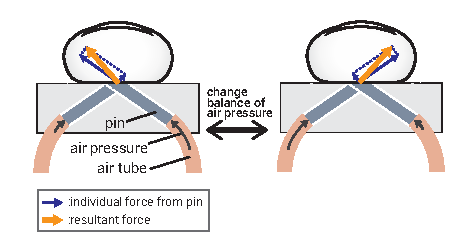
\includegraphics[width=3.4in]{images/fig_intro.eps}
  \caption{Proposed display presents the resultant force in various direction by summing individual forces from a pair of pins. We can change the direction of resultant force by only changing the air pressure on the air tubes.}
  \label{fig_intro}
\end{figure}

% 近年は装着型が多く開発されている
% Recently, more haptic system designs have started appearing with wearability in mind, and in this context wearable, pin-array displays have been developed~\cite{Koo2008, Kim2009}.
% However, currently, the ability to recognize the shape of virtual objects when using these wearable devices is worse than when users recognize real objects using a bare finger or hand.
% For example, our previous work by~\cite{taniguchi} evaluated shape recognition performance using a pin-array display covering the whole hand.
% The correct answer ratio was far inferior to the ones coming from the interaction between a real finger and the real objects, as obtained by~\cite{Klatzky1985}.

% shear方向の提示が形状認識に寄与すると思っている
% One of the promising approaches is to present not only normal force against surface but also shear force.
% The shear force should be essential for shape recognition since it provides frictional cues.
% There were studies that developed wearable display presenting shear force feedback such as \cite{Minamizawa:2007:GGW:1278280.1278289,6636291,Schorr:2017:FTD:3025453.3025744}.
% However, it is impossible to reproduce force distribution since these studies cause shear deformation of the whole skin using a pad.

